\chapter{Visualization Tools}
\label{cpt:tools}

The main contribution of this project is automatic methods for visualizing how a webcam
scene varies, and for understanding the most important variations.  In most natural
scenes, we notice changes in lighting, weather, and camera conditions which are interesting,
but fail to describe the typical behavior of a scene.  The goal of these tools is to learn 
these variations and to point out changes independent of them.  PCA is a commonly used tool, and
captures a linear model of consistent image variations.  By analyzing the results of certain PCA setups, we can obtain important and interesting information.

\section{Setup}

The most obvious way to learn about scenes is to take the PCA decomposition of the entire webcam scene.  Unfortunately, our data-set is too large for this to be feasible, so we must limit our inputs.  Instead of taking a random subset of the images, if we can intelligently limit the images we give, we can get better inputs.

\subsection{Temporal Narrowing}

The AMOS data-set consists mostly of outdoor scenes.  These outdoor scenes vary significantly over the course of a day, going from night to day and back.  The change in lighting dominates all other changes across the scene, and causes many images to be completely dark.  Instead of wasting 

\subsection{Sky Mask}

In many outdoor scenes, even when narrowed to a particular time of day, the most difficult image
variation to characterize is the sky.  PCA has a difficult time learning changes in sunlight, clouds,
and other characteristics of the sky, so this difficulty causes

Fortunately, it is fairly easy to learn which religions of an image are most affected by this challenge.

\begin{figure}
	\centering
	\subfigure[]{
		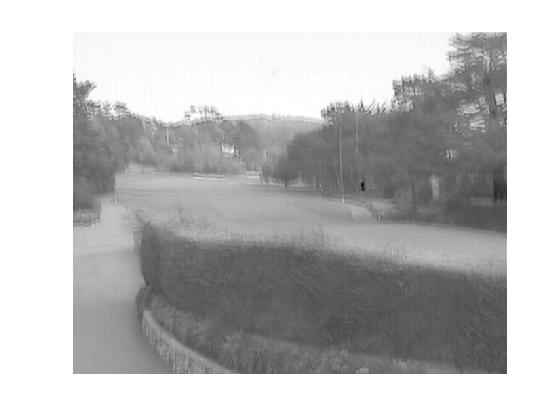
\includegraphics[width=0.45\textwidth]{figures/2skyPCA.jpg}
	\label{fig:carsNoGradient}
	}
	\subfigure[]{
		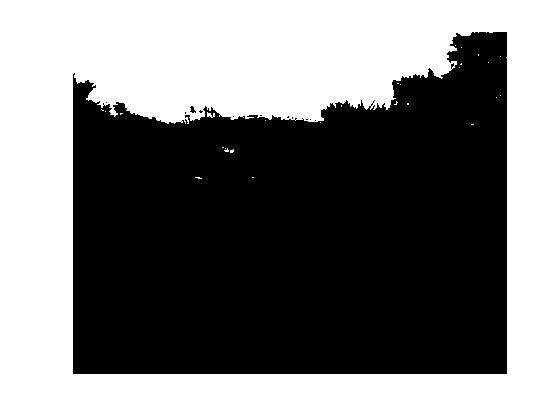
\includegraphics[width=0.45\textwidth]{figures/2skyMask.jpg}
	\label{fig:carsGradient}
	}
		\caption[Learning a sky mask for a webcam scene.]{Figure \ref{fig:2skyPCA} shows the first PCA component of a webcam scene.  By adding or subtracting this component, we control how dark or how light the sky is. Figure \ref{fig:2skyMask} shows that a simple threshholding of this image effectively segments the sky from the rest of the image.}
\end{figure}

\subsection{Gradient Image}

A webcam images are very high-dimensional - a typical 320 x 240 gray scale image has 76,800 pixels, each of
which is a value from 0 to 255.  One way to simplify this space without affecting the size of the image is to
look at the gradient magnitude images of a scene.


\begin{figure}
	\centering
	\subfigure[]{
		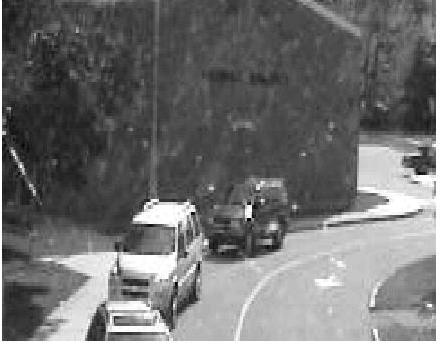
\includegraphics[width=0.45\textwidth]{figures/194cars.jpg}
	\label{fig:carsNoGradient}
	}
	\subfigure[]{
		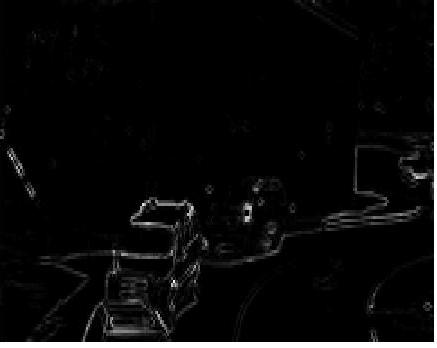
\includegraphics[width=0.45\textwidth]{figures/194carsGradient.jpg}
	\label{fig:carsGradient}
	}
		\caption[Focusing on object edges with gradient magnitude images.]{Figure \ref{fig:carsNoGradient} shows a grayscale webcam image. Figure \ref{fig:carsGradient} shows the gradient magnitude image of that frame.  Notice the noise is mostly removed and the edges are highlighted.}
\end{figure}

\section{Visualizations}

In this section, we present several tools to visualize the webcam scene based on criteria we will discuss in the next section.

% figure with a normal montage and then smart montage - potentiall from the golf scene

\subsection{Image Montage}

The simplest way to visualize a webcam scene is to view a montage of several images from that scene.  We can easily sort the images along some dimension, and then show the $n$ images with the highest values in that dimension.

\subsection{Intelligent Image Montage}

In several of these montages, we notice that many of the most unusual images are similar to each other.  This presents the problem of finding unusual images that are different from the images we have already chosen.

A simple but effective algorithm for this problem uses the L2 norm in image space.  If we consider an image as a vector of pixel intensities, such as $v = \{v_1, ..., v_m\}$, the L2 norm of two images $v$ and $u$ is $$L2\_norm(v,u) = \sqrt{\sum_{i=1}^m{(v_i-u_i)^2}}$$  Given a large set of unusual images $\{x_1, ..., x_n\}$, we compute a distance matrix $D$ where $$D_{i,j} = L2\_norm(x_i, x_j)$$  Now we iteratively find unusual images by choosing the image that has the largest distance from all of the images we have chosen so far.  Specifically, for each remaining image calculate its distance to our set of exemplars, and choose the image whose distance is the smallest.  We define the distance of an image $x_0$ to a set of exemplars $\{x_1, ..., x_n\}$ as $$d = \min_i(D(x_0, x_i))$$In this way, on each iteration, we pick the image that is least likely to be similar to an image we have already selected.  We have found that a good way to seed this process is choosing the image with the highest unusualness score as our first exemplar.

\subsection{Two-dimensional Explorer}

% figure with the 2d GUI

Using a simple GUI, we can explore a webcam scene in two dimensions.  The GUI, shown in \ref{fig:2dgui}, displays a a plot of all images on


\section{Criteria}

Once webcam scenes are projected onto a PCA basis, there are many different ways to analyze the results.
In this section, we will present several different criteria for evaluating an appearance model of a scene,
the meaning behind each criteria, and results.

\subsection{PCA coefficient vector magnitude}

For each image in a scene, PCA gives a vector of coefficients that correspond to the best linear combination
of basis images to reconstruct that image.  From this vector, we can assign each image a score equal to the
magnitude of this vector.  This gives

\subsection{Residual Error}

% figure of subplot with image, reconstruction, and residual



\subsection{Variance Model}

We can estimate the variance image of a webcam scene as the average of the square of each residual image.

One we have this variance image, we can attempt to isolate independent pixels a standard score image.

% figure with variance image, and some zScores

\subsection{Probabilistic}

We can also try to learn about an image reconstruction by treating its residual image as samples from an 
underlying probability density function.  If image deviations are due mostly to noise, we predict that these deviations will be normally distributed.

% figure showing different residual histograms

\begin{enumerate}
\item{\textbf{Normal Distribution Likelihood}}

The most obvious way to do this is to treat each residual image pixel as a sample from a normal distribution.  We can easily estimate the mean and variance of this PDF and then 

\item{\textbf{Laplacian Distribution Likelihood}}

Many of the residual images have a majority of pixels that are very close zero.  This causes the histogram to look very similar to a laplacian distribution.

\item{\textbf{Kurtosis}}

The kurtosis of a real-valued random variable is a measure of its peakedness.  Larger values of kurtosis means more variance is due to less frequent extreme deviations rather than frequent less extreme deviations.  It is defined as $$\gamma_2=\frac{\mu_4}{\sigma^4}$$ where $\mu_4$ is the fourth moment about the mean and $\sigma^4$ is the square of the variance.

We can use this measure 

\item{\textbf{Skewness}}

The skewness of a random variable is a measure of asymmetry.  Higher skewness values mean deviations on one side of the mean do not have corresponding deviations on the other side.  It is defined as $$\gamma_1=\frac{\mu_3}{\sigma^3}$$ where $\mu_3$ is the third moment about the mean and $\sigma^3$ is the cube of the standard deviation.

This measure can be used


\end{enumerate}


